\chapter{Vom Äquivalenzprinzip zu den Tensoren}

Die allgemeine Relativitätstheorie wird meist mit ART abgekürzt, obwohl die spezielle Relativitätstheorie nur selten SRT genannt wird. Wichtiger als die Abkürzung ist die Entscheidung, am Anfang anzusetzen. Der direkteste Weg ist der, den Einstein einschlug: von einer physikalischen Beobachtung auszugehen, die sich in einem Aufzug unmittelbar nachvollziehen lässt, sie so weit zu verfolgen, bis ihre Konsequenzen unausweichlich werden, und erst dann die Geometrie einzuführen.

Die erste Beobachtung ist das Äquivalenzprinzip. Gravitation und Beschleunigung sind lokal nicht zu unterscheiden. Das Wort „lokal“ wird schließlich fast die gesamte Aussage tragen. Bevor wir sie jedoch einschränken, sollten wir sehen, was sich bereits mit der uneingeschränkten Aussage erreichen lässt.

\section{Der Aufzug als Koordinatentransformation}

Lehrbücher ersetzen Einsteins Aufzug oft durch ein Raumschiff. Hier ist ein Aufzug vorzuziehen, weil seine Beschleunigung vertraut ist. Es sei \(z\) die Höhenkoordinate in einem Bezugssystem, das am Boden befestigt ist, und \(z'\) die Höhenkoordinate relativ zum Aufzugsboden. Hat der Boden die Höhe \(L(t)\), so lauten die Koordinaten desselben Ereignisses
\begin{equation}
 z'=z-L(t),\qquad t'=t,\qquad x'=x.
\label{eq:elevator-map}
\end{equation}
Die horizontale Koordinate bleibt unverändert, weil der Aufzug nicht seitwärts gleitet. Mit der bewussten Wahl \(t'=t\) wird die spezielle Relativitätstheorie zunächst ausgeklammert.

\begin{classroomqa}
\audiencequestion{Wie kann ein Kurs über allgemeine Relativitätstheorie damit beginnen, die spezielle Relativitätstheorie zu ignorieren?}
\lecturerresponse{Es gibt einen Bereich, in dem die Gravitation eine Rolle spielt, während alle Geschwindigkeiten klein gegenüber \(c\) bleiben. Der Zusammenhang zwischen Gravitation--und Beschleunigung lässt sich daher zunächst in der Newtonschen Mechanik isolieren und anschließend mit der Minkowski-Geometrie verbinden. Das ist eine Wahl für den Einstieg und keine Behauptung, die endgültige Theorie sei nichtrelativistisch. \lecturetimestamp{00:05:33}}
\end{classroomqa}

Für zwei Inertialsysteme bewegt sich der Aufzug gleichförmig:
\begin{equation}
 L(t)=vt,\qquad z'=z-vt.
\label{eq:galilean-elevator}
\end{equation}
Die Ursprünge wurden so gewählt, dass sie bei \(t=0\) zusammenfallen. Auf der Tafel bleibt die Aufzugsskizze neben allen drei Koordinatenbeziehungen stehen, damit die Symbole stets ihre physikalische Bedeutung behalten.

\begin{figure}[H]
\centering
\includegraphics[width=\linewidth]{lecture_01_figure_01.png}
\caption{Die Aufzugskoordinaten im Spezialfall gleichförmiger Bewegung \(L(t)=vt\).}
\par\smallskip
\textit{Vorlesungsbild: 00:09:10.}
\end{figure}

Betrachten wir nur die vertikale Komponente des Newtonschen Gesetzes:
\begin{equation}
 F=m\ddot z.
\label{eq:newton-unprimed}
\end{equation}
Die Kraft kann von einem Seil, einem elektrischen Feld oder einer anderen gewöhnlichen Wechselwirkung stammen. Zweimaliges Ableiten von \eqref{eq:galilean-elevator} ergibt
\(\ddot z'=\ddot z\) und damit
\begin{equation}
 F=m\ddot z'.
\label{eq:newton-primed-inertial}
\end{equation}
Die Form des Gesetzes bleibt unverändert. Diese elementare Rechnung macht den entscheidenden Gehalt der Äquivalenz von Inertialsystemen sichtbar: Eine lineare Koordinatentransformation bildet gleichförmige Bewegung auf gleichförmige Bewegung ab.

\begin{figure}[H]
\centering
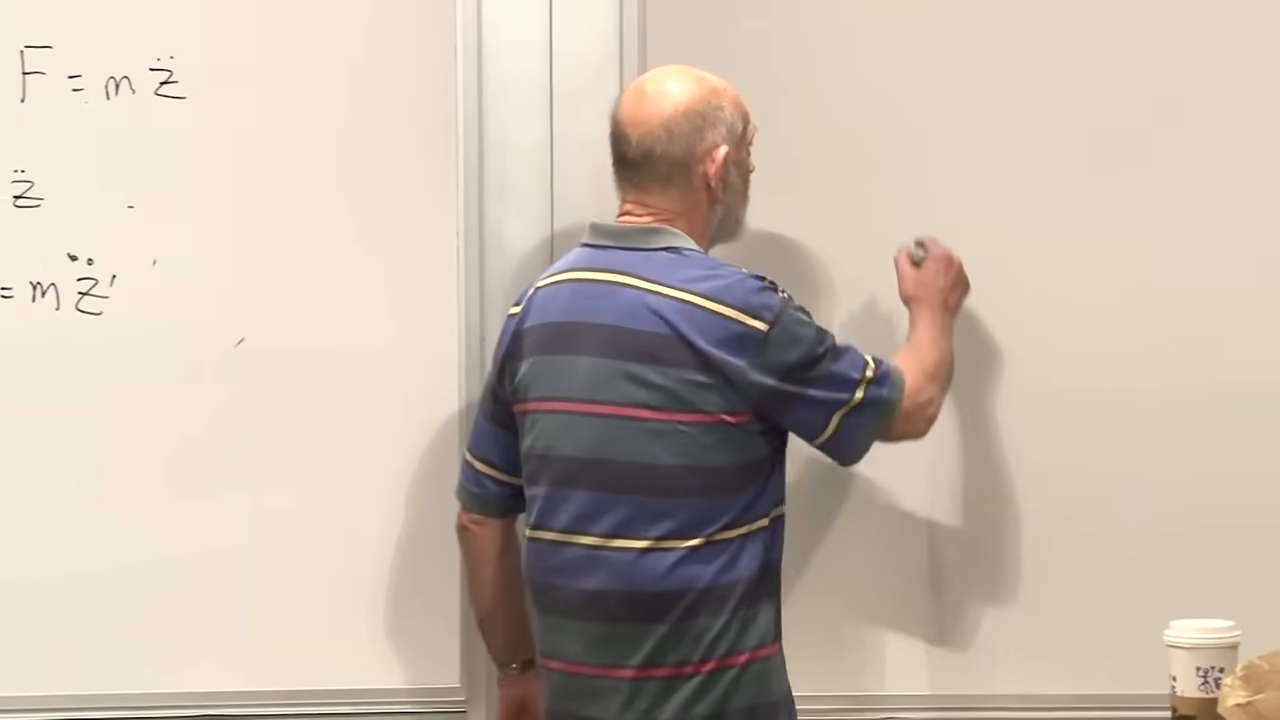
\includegraphics[width=\linewidth]{lecture_01_figure_02.png}
\caption{Die Newtonsche Gleichung in zwei gleichförmig gegeneinander bewegten Koordinatensystemen.}
\par\smallskip
\textit{Vorlesungsbild: 00:11:50.}
\end{figure}

Beschleunigen wir den Aufzug nun mit konstanter Beschleunigung \(g\) nach oben:
\begin{equation}
 L(t)=\frac12gt^2,\qquad
 \dot L=gt,\qquad
 \ddot L=g.
\end{equation}
Die Koordinatentransformation lautet dann
\begin{equation}
 z'=z-\frac12gt^2,
\qquad
 \ddot z'=\ddot z-g.
\label{eq:accelerated-map}
\end{equation}
Einsetzen in das Newtonsche Gesetz ergibt
\begin{equation}
 F=m(\ddot z'+g),
\qquad
 m\ddot z'=F-mg.
\label{eq:fictitious-gravity}
\end{equation}
Bei der Herleitung lässt sich das Vorzeichen gut unmittelbar überprüfen: \(+mg\) steht zunächst auf der Beschleunigungsseite und wird erst beim Verschieben auf die Kraftseite zu \(-mg\). Im Bezugssystem, dessen Boden nach oben beschleunigt, zeigt die resultierende Richtung nach unten.

\begin{figure}[H]
\centering
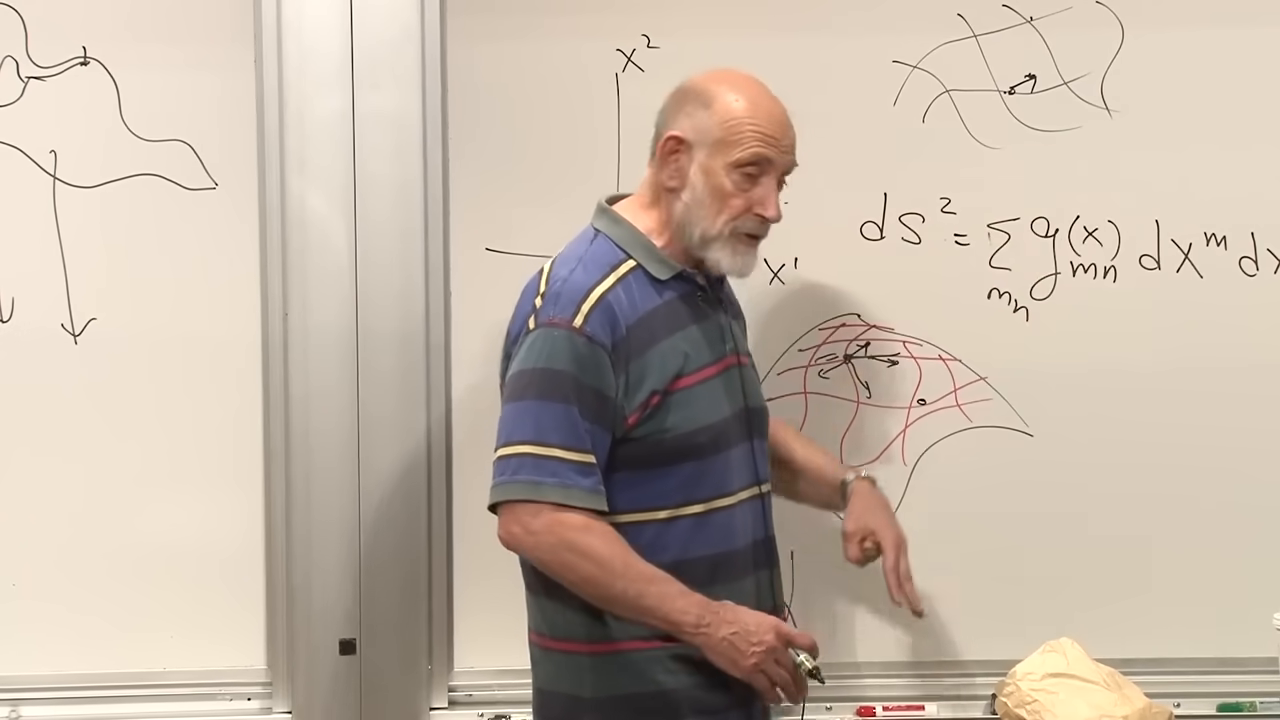
\includegraphics[width=\linewidth]{lecture_01_figure_03.png}
\caption{Die beschleunigte Transformation und die daraus folgende Scheinkraft \(-mg\).}
\par\smallskip
\textit{Vorlesungsbild: 00:15:35.}
\end{figure}

Der neue Term sieht aus einem präzisen Grund wie Gravitation aus: Er ist proportional zur Masse. Da auch die Trägheitsreaktion proportional zur Masse ist, kürzt sich die Masse in der Bewegungsgleichung heraus. Ein frei fallender Körper folgt unabhängig von seiner Masse derselben Bahn. Die Erdbahn wird zum Beispiel in der Näherung eines Probekörpers durch dessen Position und Geschwindigkeit im Gravitationsfeld der Sonne bestimmt, nicht durch die eigene Masse der Erde.

Vor Einstein hätte man diese Ähnlichkeit als Kuriosität abtun können. Einstein erhob sie stattdessen zum Prinzip: Kein lokales mechanisches Experiment kann ein homogenes Gravitationsfeld von einem passend beschleunigten Bezugssystem unterscheiden.

\section{Geraden, gekrümmte Koordinaten und Licht}

Tragen wir \(t\) vertikal und \(z\) horizontal auf. Für \(z'=z-vt\) sind die Linien konstanter \(z'\) parallele Geraden. Geradlinige Weltlinien bleiben gerade, weil die Koordinatentransformation linear ist.

\begin{figure}[H]
\centering
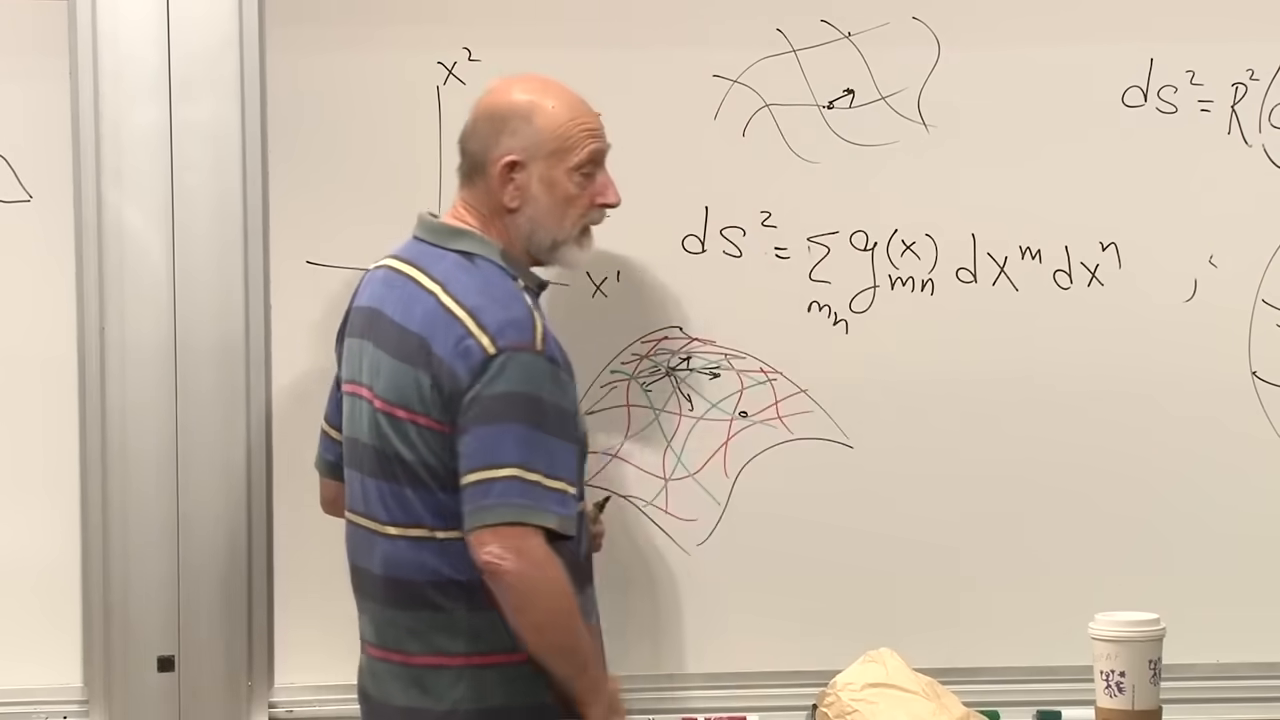
\includegraphics[width=\linewidth]{lecture_01_figure_04.png}
\caption{Ein lineares Raumzeitgitter für gleichförmig bewegte Koordinaten.}
\par\smallskip
\textit{Vorlesungsbild: 00:19:45.}
\end{figure}

Bei der beschleunigten Abbildung erfüllt eine Linie konstanten \(z'\) die Gleichung
\begin{equation}
 z=z'+\frac12gt^2.
\end{equation}
Sie ist eine seitlich liegende Parabel. Verlängert man die Bewegung rückwärts in der Zeit, so sinkt der Aufzug zunächst langsamer werdend ab, kehrt dann um und beschleunigt anschließend nach oben. Jede benachbarte Linie mit konstantem \(z'\) ist dieselbe Parabel, nur horizontal verschoben.

\begin{figure}[H]
\centering
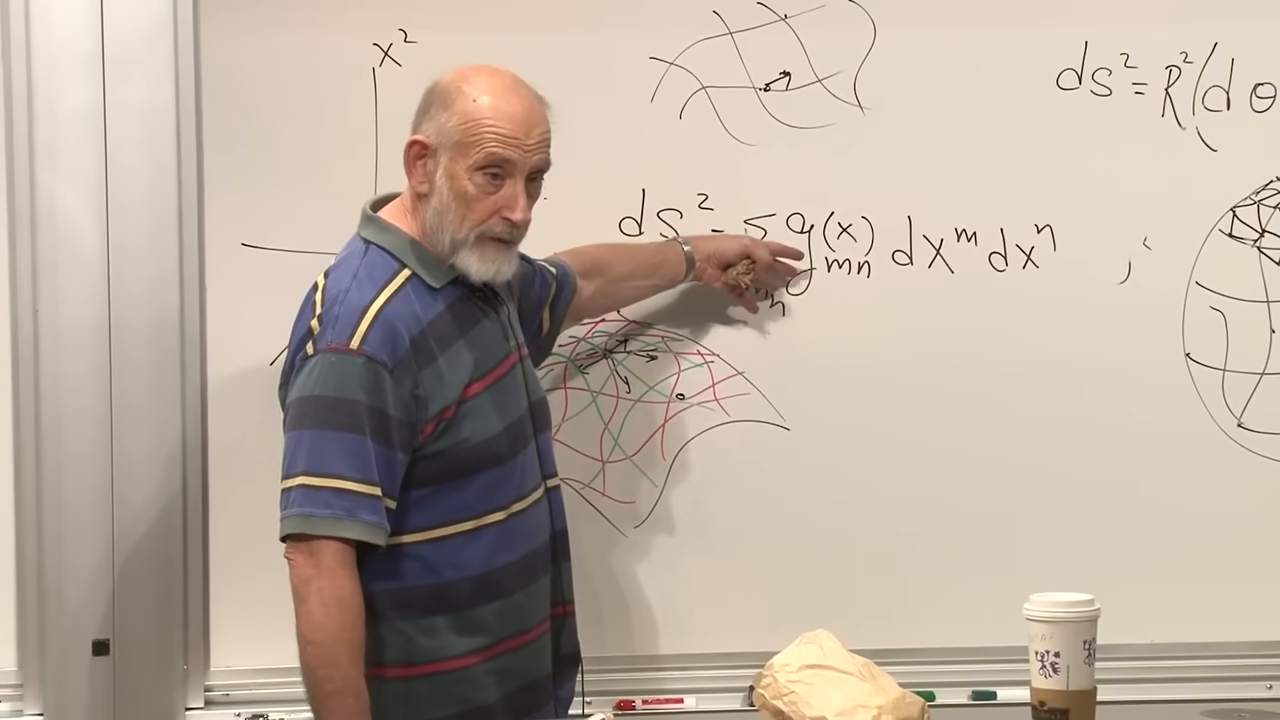
\includegraphics[width=\linewidth]{lecture_01_figure_05.png}
\caption{Kurven konstanten \(z'\) für das gleichmäßig beschleunigte Koordinatensystem.}
\par\smallskip
\textit{Vorlesungsbild: 00:22:25.}
\end{figure}

Das ist der erste geometrische Hinweis. In der speziellen Relativitätstheorie bilden lineare Lorentz-Transformationen gerade Raumzeitlinien auf gerade Raumzeitlinien ab. Um Beschleunigung und damit Gravitation nachzubilden, braucht man krummlinige Transformationen der Raumzeitkoordinaten.

Einstein nutzte diesen scheinbar bescheidenen Punkt, um eine alles andere als bescheidene Frage zu beantworten: Beeinflusst Gravitation das Licht? Bei \(t=0\) seien Aufzug und Bodenbezugssystem momentan relativ zueinander in Ruhe; dann schicken wir einen horizontalen Lichtstrahl durch den Aufzug. Im unbeschleunigten Bezugssystem gilt
\begin{equation}
 x=ct,\qquad z=0.
\end{equation}
Mit \(z=z'+\tfrac12gt^2\) erfüllt derselbe Strahl in den Aufzugskoordinaten die Gleichung
\begin{equation}
 z'=-\frac12gt^2
    =-\frac{g}{2c^2}x^2.
\label{eq:accelerated-light}
\end{equation}
Im Inertialsystem verläuft der Lichtstrahl gerade, im beschleunigten Bezugssystem dagegen gekrümmt. Sind Beschleunigung und Gravitation lokal äquivalent, muss ein Gravitationsfeld Licht ablenken. Die Argumentation zeigt diesen Effekt, bevor überhaupt eine Feldgleichung für die Gravitation aufgestellt wurde.

\begin{figure}[H]
\centering
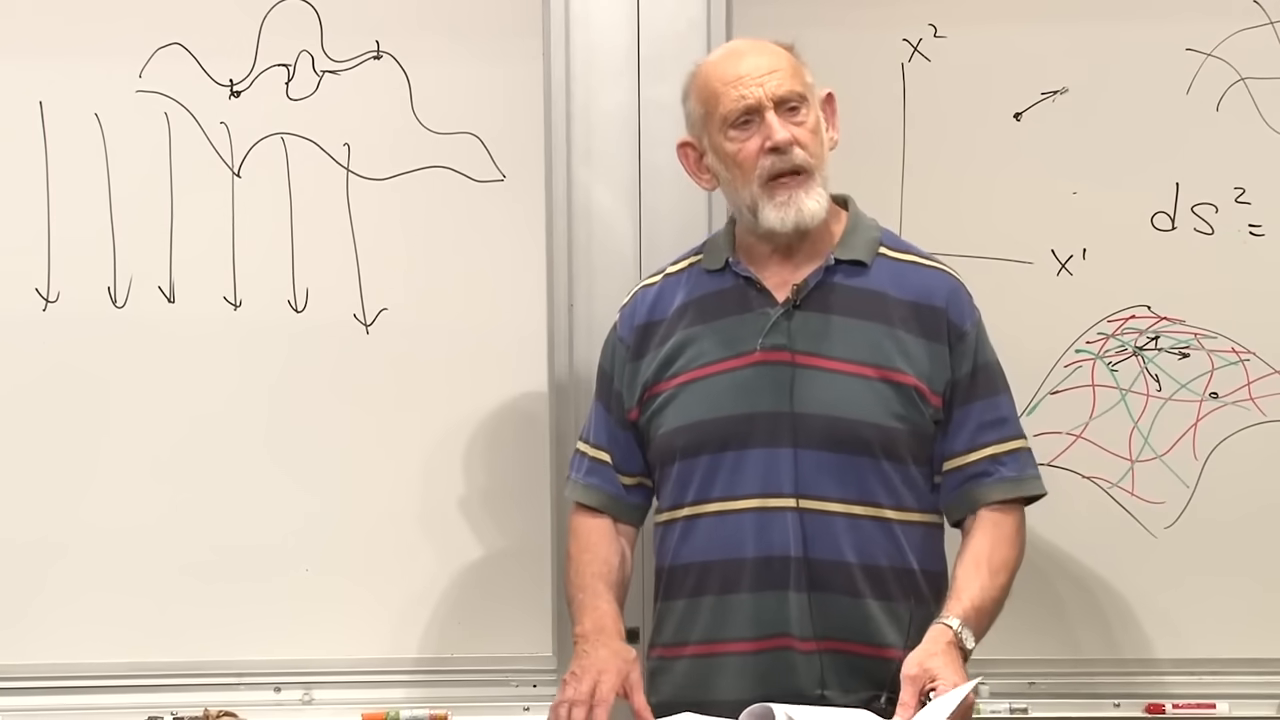
\includegraphics[width=\linewidth]{lecture_01_figure_06.png}
\caption{Der horizontale Lichtstrahl und seine gekrümmte Bahn im beschleunigten Bezugssystem.}
\par\smallskip
\textit{Vorlesungsbild: 00:28:10.}
\end{figure}

\section{Was sich nicht wegtransformieren lässt}

Ein beschleunigtes Bezugssystem kann ein scheinbares homogenes Gravitationsfeld erzeugen. Daraus folgt nicht, dass jedes Gravitationsfeld ein Koordinatenartefakt ist. Das Feld eines Sterns zeigt radial nach innen. Ein kleines, frei fallendes Labor in der Nähe eines einzelnen Punktes kann die lokale Beschleunigung beseitigen, aber dieselbe Transformation kann das Feld nicht auf allen Seiten des Sterns beseitigen.

\begin{figure}[H]
\centering
\includegraphics[width=\linewidth]{lecture_01_figure_07.png}
\caption{Ein Radialfeld und ein ausgedehnter fallender Körper machen die Gezeitenbeschleunigung sichtbar.}
\par\smallskip
\textit{Vorlesungsbild: 00:32:50.}
\end{figure}

Das Hindernis ist die Gezeitenkraft. Stellen wir uns eine zweitausend Meilen große Person vor, die mit den Füßen voraus fällt. Ihre Füße sind der Quelle näher und werden stärker beschleunigt als ihr Kopf, sodass sie gedehnt wird. Dreht sie sich auf die Seite, so haben die nach innen gerichteten Kräfte auf den gegenüberliegenden Seiten Komponenten, die aufeinander zuweisen; sie wird also zusammengedrückt. In Newtonscher Sprache erfahren benachbarte Punkte mit Abstand \(\xi^j\) eine Relativbeschleunigung
\begin{equation}
 \delta a^i \simeq \partial_j g^i\,\xi^j.
\label{eq:newtonian-tide}
\end{equation}
Eine Koordinatenbeschleunigung lässt sich beseitigen. Die Relativbeschleunigung über einen ausgedehnten frei fallenden Körper hinweg lässt sich nicht beseitigen.

\begin{classroomqa}
\audiencequestion{Könnten unterschiedlich starke Raketentriebwerke an Kopf und Füßen die Dehnung nachbilden und damit ein Gezeitenfeld simulieren?}
\lecturerresponse{Triebwerke können einen Körper durchaus belasten, doch dabei wirkt eine reale, nichtgravitative Kraft unterschiedlich auf seine Teile. Eine bloße Koordinatenänderung kann keine invariante Relativbeschleunigung benachbarter frei fallender Teilchen erzeugen. Das Diagnoseverfahren betrifft den freien Fall ohne äußere Kräfte, nicht einen Körper, der von getrennten Raketen angetrieben wird.
\lecturetimestamp{00:36:51}}
\end{classroomqa}

Gekrümmte Koordinaten können dennoch sehr komplizierte Scheinfelder erzeugen. Ein Bezugssystem kann vertikal beschleunigen und zugleich horizontal schwingen, sodass ein zeitabhängiges scheinbares Feld mit Komponenten in beiden Richtungen entsteht. Auch gewöhnliche Polarkoordinaten liefern ein anschauliches Beispiel. Ein freies Teilchen, das sich geradlinig in kartesischen Koordinaten bewegt, hat zunächst einen abnehmenden Wert von \(r(t)\), erreicht einen minimalen Radius und dann einen zunehmenden Wert von \(r(t)\). Wer nur \(r(t)\) und \(\theta(t)\) kennt, könnte daraus auf eine nach außen gerichtete abstoßende Kraft schließen. Bei rotierenden Varianten dieser Koordinaten treten Zentrifugal- und Coriolisterme auf. Sie sind proportional zur Masse und sehen daher wie Gravitation aus, hinterlassen aber keine invariante Gezeitendeformation an einem frei fallenden Körper.

\begin{classroomqa}
\audiencequestion{Was passiert, wenn die Bewegung in Winkel- oder Polarkoordinaten beschrieben wird?}
\lecturerresponse{Die nichtlineare Koordinatenbeschreibung lässt eine geradlinige freie Bahn so erscheinen, als werde das Teilchen von \(r=0\) abgestoßen. Diese effektive Zentrifugalkraft ist eine Koordinatenkraft. Die Rückkehr zu einem inertialen kartesischen Bezugssystem beseitigt sie und zeigt, dass keine Gezeitendeformation vorliegt.
\lecturetimestamp{00:37:56}}
\end{classroomqa}

\begin{figure}[H]
\centering
\includegraphics[width=\linewidth]{lecture_01_figure_08.png}
\caption{Die Beschreibung einer geradlinigen Bahn in Polarkoordinaten; \(r(t)\) und \(\theta(t)\) sind an der Tafel markiert.}
\par\smallskip
\textit{Vorlesungsbild: 00:40:20.}
\end{figure}

\begin{classroomqa}
\audiencequestion{Können mehrere gravitative Körper einander aufheben, sodass keine Gezeitenkraft übrig bleibt?}
\lecturerresponse{Kräfte können sich an einem bestimmten Punkt aufheben, doch die Aufhebung des Feldwerts hebt seine räumlichen Ableitungen im Allgemeinen nicht auf. In der Nähe jeder einzelnen Quelle erfahren benachbarte Bahnen weiterhin unterschiedliche Beschleunigungen. Damit Krümmung wirklich fehlt, muss das Gezeitenkriterium im gesamten Gebiet verschwinden, nicht nur die resultierende Kraft an einem Punkt. \lecturetimestamp{00:42:16}}
\end{classroomqa}

\begin{classroomqa}
\audiencequestion{Wie lässt sich eine Gezeitenkraft operational messen?}
\lecturerresponse{Man lässt einen ausgedehnten Gegenstand, etwa einen Kristall, frei fallen und untersucht, ob Spannungen und Dehnungen ihn in einer Richtung strecken und in einer anderen zusammendrücken. Diese Verformungen sind messbar und verschwinden nicht, wenn man die Koordinaten umbenennt. \lecturetimestamp{00:44:38}}
\end{classroomqa}

\begin{classroomqa}
\audiencequestion{Würde eine zweitausend Meilen große Person auf einem Karussell eine radiale Gezeitenwirkung spüren?}
\lecturerresponse{Eine auf dem Karussell festgeschnallte Person spürt Stützkräfte und bekommt womöglich tatsächlich Kopfschmerzen. Der Testkörper muss stattdessen frei fallen. In rotierenden Koordinaten sieht seine Bahn kompliziert aus, aber im Inertialsystem bleibt sie eine unverformte gerade Bahn; die invariante Gezeitenkraft ist daher null.
\lecturetimestamp{00:45:07}}
\end{classroomqa}

\begin{classroomqa}
\audiencequestion{Kann man den fallenden Körper so neigen, dass sich Dehnung und Zusammendrückung aufheben?}
\lecturerresponse{Keine einzelne Ausrichtung beseitigt die gesamte Verformung. Das Radialfeld dehnt in einer Hauptrichtung und drückt in den dazu quer verlaufenden Richtungen zusammen. Ein Körper mit endlicher Ausdehnung in allen Richtungen erfährt das vollständige Muster. \lecturetimestamp{00:47:10}}
\end{classroomqa}

\begin{figure}[H]
\centering
\includegraphics[width=\linewidth]{lecture_01_figure_09.png}
\caption{Radiale Dehnung und transversale Zusammendrückung gemeinsam dargestellt an einem ausgedehnten frei fallenden Körper.}
\par\smallskip
\textit{Vorlesungsbild: 00:47:55.}
\end{figure}

\begin{classroomqa}
\audiencequestion{Bedeuten Gezeitenkräfte, dass das Äquivalenzprinzip versagt?}
\lecturerresponse{Sie bestimmen, wie sorgfältig das Prinzip formuliert werden muss. In einem System, das klein genug ist, dass sich das Gravitationsfeld darin vernachlässigbar wenig ändert, lässt sich die Gravitation mit der erforderlichen Genauigkeit durch ein frei fallendes Bezugssystem beseitigen. Die verbleibende Änderung über ein größeres System hinweg ist das Gezeitenfeld. \lecturetimestamp{00:48:08}}
\end{classroomqa}

\section{Von der Minkowski-Geometrie zu einer lokalen Metrik}

Nun wenden wir uns vorübergehend von der Gravitation ab. Minkowski hatte bereits gezeigt, dass die Raumzeit eine invariante lokale Geometrie besitzt. In einer Raumdimension und mit \(c=1\) gilt
\begin{equation}
 d\tau^2=dt^2-dx^2.
\label{eq:minkowski-proper-time}
\end{equation}
Stattdessen kann man auch \(ds^2=dx^2-dt^2=-d\tau^2\) definieren. Der Unterschied betrifft die Vorzeichenkonvention, nicht die Physik.

\begin{classroomqa}
\audiencequestion{Wo kommt die Lichtgeschwindigkeit vor, wenn sie nicht gleich eins gesetzt wird?}
\lecturerresponse{Wird \(t\) in Zeiteinheiten und \(x\) in Längeneinheiten gemessen, ist folgende Form praktisch:
\(d\tau^2=dt^2-dx^2/c^2\). Äquivalent dazu kann man mit \(c^2\) multiplizieren und \(c^2d\tau^2=c^2dt^2-dx^2\) verwenden. Mit der Wahl von \(ct\) oder \(x/c\) als Koordinate wird der Umrechnungsfaktor absorbiert. \lecturetimestamp{00:51:02}}
\end{classroomqa}

\begin{figure}[H]
\centering
\includegraphics[width=\linewidth]{lecture_01_figure_10.png}
\caption{Das Eigenzeitintervall liefert die geometrische Verbindung von der speziellen zur allgemeinen Relativitätstheorie.}
\par\smallskip
\textit{Vorlesungsbild: 00:51:10.}
\end{figure}

Einstein erkannte, dass die Frage, ob ein Gravitationsfeld beseitigt werden kann, einem Problem ähnelt, das Gauß für Flächen und Riemann für beliebige Dimensionen untersucht hatten: Wie lässt sich aus einem lokalen Abstandsmaß bestimmen, ob die Geometrie tatsächlich gekrümmt ist?

In euklidischen kartesischen Koordinaten liefert der Satz des Pythagoras
\begin{equation}
 ds^2=(dx^1)^2+(dx^2)^2+\cdots
     =\delta_{mn}\,dx^m dx^n.
\label{eq:euclidean-line-element}
\end{equation}
Der Indexbereich entspricht der Dimension des Raums. An der Notation ändert sich nichts, gleichgültig, ob es zwei, drei oder sechsundzwanzig Koordinaten gibt.

\begin{figure}[H]
\centering
\includegraphics[width=\linewidth]{lecture_01_figure_11.png}
\caption{Das euklidische Linienelement als Summe quadrierter Koordinatendifferentiale.}
\par\smallskip
\textit{Vorlesungsbild: 00:55:00.}
\end{figure}

Wählen wir beliebige Koordinaten \(x^m\) auf einer beliebigen Fläche. Der Abstand zwischen benachbarten Punkten ist durch die quadratische Form gegeben:
\begin{equation}
 ds^2=g_{mn}(x)\,dx^m dx^n.
\label{eq:general-line-element}
\end{equation}
Die Funktionen \(g_{mn}(x)\) sind die Komponenten des metrischen Tensors. Dieselbe Formel gilt auch für eine flache Fläche, die mit krummlinigen Koordinaten beschrieben wird; nicht konstante Metrikkomponenten allein beweisen keine intrinsische Krümmung.

\begin{figure}[H]
\centering
\includegraphics[width=\linewidth]{lecture_01_figure_12.png}
\caption{Eine allgemeine metrische quadratische Form neben einem gekrümmten Koordinatennetz.}
\par\smallskip
\textit{Vorlesungsbild: 00:58:20.}
\end{figure}

Für eine Kugel mit Radius \(R\) gilt, wenn \(\theta\) vom Pol aus gemessen wird:
\begin{equation}
 ds^2=R^2\left(d\theta^2+\sin^2\theta\,d\phi^2\right).
\label{eq:sphere-polar}
\end{equation}
Ein und dasselbe Längengradintervall entspricht am Äquator einer großen und in Polnähe einer kleinen Strecke. Genau diese Positionsabhängigkeit erfasst der Koeffizient.

\begin{classroomqa}
\audiencequestion{Die gewöhnliche geografische Breite wird vom Äquator aus gemessen. Müsste der Koeffizient dann nicht ein Kosinus statt eines Sinus sein?}
\lecturerresponse{Ja. Bezeichnet \(\lambda\) die vom Äquator aus gemessene geografische Breite, so gilt
\(ds^2=R^2(d\lambda^2+\cos^2\lambda\,d\phi^2)\).
In Gleichung \eqref{eq:sphere-polar} wird der vom Nordpol aus gemessene Polarwinkel \(\theta=\pi/2-\lambda\) verwendet.
\lecturetimestamp{01:01:03}}
\end{classroomqa}

\begin{figure}[H]
\centering
\includegraphics[width=\linewidth]{lecture_01_figure_13.png}
\caption{Die Kugelmetrik und die Geometrie aus Breiten--Längengraden, die ihren ortsabhängigen Koeffizienten festlegt.}
\par\smallskip
\textit{Vorlesungsausschnitt: 01:00:30.}
\end{figure}

Allgemeinere Koordinaten können \(d\theta\,d\phi\)-Mischterme enthalten, doch das lokale Abstandsmaß bleibt eine quadratische Form in den Differentialen. Kubische oder lineare Terme gehören nicht in ein Riemannsches Linienelement.

\section{Lokale Abstände und intrinsische Krümmung}

\begin{classroomqa}
\audiencequestion{Liefert die Metrikformel auch den Abstand zwischen zwei weit voneinander entfernten Punkten?}
\lecturerresponse{Nicht durch direktes Einsetzen. Sie liefert den Abstand zwischen benachbarten Punkten. Für einen Abstand über eine makroskopische Strecke braucht man einen Weg und ein Integral über \(ds\); ist mit dem Abstand der kürzeste Weg gemeint, muss dieser Weg anhand der Geometrie selbst bestimmt werden. Sogar mehrere lokal kürzeste Wege können dieselben Endpunkte verbinden. \lecturetimestamp{01:02:30}}
\end{classroomqa}

Stellen wir uns auf einer unebenen Fläche zwei Pflöcke an weit auseinanderliegenden Punkten und eine gespannte Schnur dazwischen vor. Die Schnur kann auf der einen oder der anderen Seite eines Hügels verlaufen; verändert man den Hügel, ändert sich der kürzeste Weg. Der globale Abstand hängt von der Geometrie dazwischen ab. Der lokale Abstand ist einfacher: Die Metrik liefert an jedem Punkt ein kleines Messstäbchen, und aus diesen infinitesimalen Stäbchen setzt sich die Geometrie zusammen.

\begin{figure}[H]
\centering
\includegraphics[width=\linewidth]{lecture_01_figure_14.png}
\caption{Das Problem des globalen Abstands: Ein gespannter Weg muss sich zwischen den Endpunkten der Fläche anpassen.}
\par\smallskip
\textit{Vorlesungsbild: 01:04:00.}
\end{figure}

Lassen sich die lokalen Stücke ohne Dehnung oder Risse auf eine Ebene legen, ist die intrinsische Geometrie flach. Stücke mit den Seitenlängen einer triangulierten Kugel lassen sich nicht alle unter Beibehaltung ihrer Kantenlängen flach auslegen. Die Metrik stellt damit eine präzise Frage: Lässt sich anhand von \(g_{mn}(x)\) bestimmen, ob sich die infinitesimalen Stücke zu einem flachen Raum zusammenfügen?

\begin{figure}[H]
\centering
\includegraphics[width=\linewidth]{lecture_01_figure_15.png}
\caption{Die Metrik und ein lokaler Koordinatenbereich, aufgefasst als infinitesimale Stücke, aus denen die Geometrie zusammengesetzt ist.}
\par\smallskip
\textit{Vorlesungsbild: 01:05:20.}
\end{figure}

\begin{classroomqa}
\audiencequestion{Kann man die Krümmung diagnostizieren, indem man das Verhältnis von Umfang zu Durchmesser misst?}
\lecturerresponse{Ja, das ist ein nützlicher Test in zwei Dimensionen. Auf einer gekrümmten Fläche kann das Verhältnis von \(\pi\) abweichen. Bei einem infinitesimal kleinen Kreis tritt die Abweichung allerdings erst in höherer Ordnung auf, und die Methode lässt sich nicht so unmittelbar verallgemeinern wie ein Krümmungstensor.
\lecturetimestamp{01:07:26}}
\end{classroomqa}

Ein Gebiet ist flach, wenn es ein Koordinatensystem gibt, in dem
\begin{equation}
 g_{mn}=\delta_{mn},
\qquad
 ds^2=\delta_{mn}\,dx^m dx^n
\label{eq:flat-metric}
\end{equation}
im gesamten Gebiet gilt. Eine komplizierte Metrik \(g_{mn}(x)\) kann daher entweder einen gekrümmten Raum beschreiben oder lediglich gekrümmte Koordinaten in einem flachen Raum. Entscheidend ist, ob sich die gesamte Kompliziertheit durch eine Koordinatentransformation beseitigen lässt.

\begin{figure}[H]
\centering
\includegraphics[width=\linewidth]{lecture_01_figure_16.png}
\caption{Das Metrikproblem auf einem lokalen Koordinatenbereich: Lässt sich ihre krummlinige Form in die flache Form transformieren?}
\par\smallskip
\textit{Vorlesungsbild: 01:07:15.}
\end{figure}

\begin{classroomqa}
\audiencequestion{Setzt das Linienelement der Kugel voraus, dass jedes kleine Intervall flach ist, obwohl die Kugel gekrümmt ist?}
\lecturerresponse{In führender Ordnung lässt sich jede glatte Fläche an einem Punkt durch ihre Tangentialebene annähern. Krümmung zeigt sich darin, dass benachbarte Tangentialebenen nicht genau zusammenpassen, oder in Änderungen höherer Ordnung über einen endlichen Bereich hinweg. Lokales euklidisches Verhalten und globale Krümmung sind daher miteinander vereinbar. \lecturetimestamp{01:10:01}}
\end{classroomqa}

\begin{classroomqa}
\audiencequestion{Muss die Metrik stetig sein, und was geschieht an einer Falte oder in einer Vertiefung?}
\lecturerresponse{Die Betrachtung setzt voraus, dass Koordinatenabbildungen und Metrik für die benötigten Ableitungen hinreichend glatt sind. Ein ohne Dehnung gefaltetes Blatt hat auf beiden Seiten der Falte dieselben intrinsischen Abstände; sein auffälliges Erscheinungsbild ist extrinsisch. Eine tatsächlich singuläre oder nicht glatte Geometrie erfordert eine gesonderte Behandlung und liegt außerhalb des hier verwendeten glatten Rahmens. \lecturetimestamp{01:11:25}}
\end{classroomqa}

Dieser Unterschied betrifft die intrinsische Geometrie. Wird eine Seite im dreidimensionalen Raum gebogen, ändert sich ihre Einbettung, aber nicht die Abstände innerhalb der Seite. Ein Lebewesen, das auf die Seite beschränkt ist und nicht in den Einbettungsraum hinaussehen kann, kann ihre intrinsische Geometrie dennoch messen.

\begin{figure}[H]
\centering
\includegraphics[width=\linewidth]{lecture_01_figure_17.png}
\caption{Ein gefaltetes Blatt veranschaulicht den Unterschied zwischen intrinsischem Abstand und extrinsischem Erscheinungsbild.}
\par\smallskip
\textit{Vorlesungsbild: 01:13:00.}
\end{figure}

\begin{classroomqa}
\audiencequestion{Warum diagonalisiert man die Metrik nicht einfach?}
\lecturerresponse{An jedem einzelnen Punkt lässt sich die Metrik durch eine geeignete Koordinatenwahl diagonalisieren und auf die lokale flache Form normieren. Die Schwierigkeit besteht darin, das in einem ganzen Gebiet mit einem einzigen Koordinatensystem zu erreichen. Krümmung lässt sich nicht allein durch Untersuchung eines einzelnen Punktes feststellen.
\lecturetimestamp{01:13:48}}
\end{classroomqa}

\begin{figure}[H]
\centering
\includegraphics[width=\linewidth]{lecture_01_figure_18.png}
\caption{Die flache kartesische Metrik \(\delta_{mn}\) unter der allgemeinen lokalen quadratischen Form dargestellt.}
\par\smallskip
\textit{Vorlesungsausschnitt: 01:16:00.}
\end{figure}

Die Analogie zur Gravitation ist nun exakt und nicht länger nur ein Hinweis. Eine Koordinatenkraft lässt sich ebenso beseitigen wie eine krummlinige Beschreibung des flachen Raums. In der allgemeinen Relativitätstheorie wird Gezeitenbeschleunigung durch Krümmung beschrieben. In späterer Notation erfüllen benachbarte, frei fallende Weltlinien die Gleichung der geodätischen Abweichung:
\begin{equation}
 \frac{D^2\xi^\mu}{D\tau^2}
 =-R^\mu{}_{\nu\rho\sigma}
   u^\nu\xi^\rho u^\sigma.
\label{eq:geodesic-deviation-preview}
\end{equation}
Verschwindet die Krümmung, gibt es kein invariantes Gezeitenfeld; ist sie ungleich null, kann keine Koordinatenwahl die Gravitation im ganzen Gebiet beseitigen.

\section{Zwei Koordinatensysteme und ein Vektor}

Um zu entscheiden, ob sich eine Metrik in \(\delta_{mn}\) transformieren lässt, müssen wir zunächst wissen, wie geometrische Objekte transformieren. Seien \(x^m\) und \(y^m\) zwei glatte Koordinatensysteme in demselben Gebiet:
\begin{equation}
 x^m=x^m(y),\qquad y^m=y^m(x).
\label{eq:mutual-coordinate-maps}
\end{equation}
Die Symbole \(x\) und \(y\) bezeichnen vollständige Koordinatensysteme, nicht zwei bestimmte Raumrichtungen.

\begin{figure}[H]
\centering
\includegraphics[width=\linewidth]{lecture_01_figure_19.png}
\caption{Die einander zugeordneten Koordinatenabbildungen \(x^m(y)\) und
\(y^m(x)\).}
\par\smallskip
\textit{Vorlesungsausschnitt: 01:20:35.}
\end{figure}

Für benachbarte Punkte ergibt sich aus der Kettenregel
\begin{equation}
 dy^m=\frac{\partial y^m}{\partial x^p}\,dx^p.
\label{eq:differential-transform}
\end{equation}
Der wiederholte Index \(p\) wird summiert. Die Verschiebung selbst ist ein einziger geometrischer Vektor; \(dx^p\) und \(dy^m\) sind seine Komponenten in zwei Koordinatensystemen.

\begin{figure}[H]
\centering
\includegraphics[width=\linewidth]{lecture_01_figure_20.png}
\caption{Die differentielle Koordinatentransformation, hergeleitet mithilfe der Kettenregel.}
\par\smallskip
\textit{Vorlesungsbild: 01:22:30.}
\end{figure}

\begin{classroomqa}
\audiencequestion{Was stellen die Koordinatenlinien in einem krummlinigen Gitter dar?}
\lecturerresponse{In zwei Dimensionen erhält man eine Linie, indem man eine Koordinate festhält und die andere variiert. In höheren Dimensionen entsprechen dem Hyperflächen mit konstanten Koordinaten. Ihre lokalen Schnittmengen legen die Koordinatenrichtungen fest, entlang derer Vektorkomponenten angegeben werden. \lecturetimestamp{01:25:20}}
\end{classroomqa}

Ein kontravarianter Vektor ist durch dasselbe Transformationsgesetz wie eine Koordinatenverschiebung definiert:
\begin{equation}
 (V')^m(y)
 =\frac{\partial y^m}{\partial x^p}\,V^p(x).
\label{eq:contravariant-vector}
\end{equation}
Die Geschwindigkeit entlang einer Fläche ist ein Beispiel. Bei einem Koordinatenwechsel ändert sich der Vektor nicht, wohl aber seine Komponenten.

\begin{figure}[H]
\centering
\includegraphics[width=\linewidth]{lecture_01_figure_21.png}
\caption{Das eingerahmte Transformationsgesetz für einen kontravarianten Vektor.}
\par\smallskip
\textit{Vorlesungsbild: 01:29:30.}
\end{figure}

Nach Einsteins Summenkonvention lässt man das Summenzeichen weg, wenn ein Index einmal oben und einmal unten wiederholt wird. Die Konvention erleichterte den Formeldruck; wichtiger noch: Sie macht das Kontraktionsmuster sichtbar.

\begin{classroomqa}
\audiencequestion{Gibt es bestimmte Annahmen darüber, welche Koordinatensysteme zulässig sind?}
\lecturerresponse{Es wird lediglich vorausgesetzt, dass die beiden Systeme funktional zusammenhängen und hinreichend glatt sind, sodass die dargestellten Ableitungen und die inverse Abbildung im betrachteten Gebiet existieren. Weder Linearität noch Orthogonalität wird vorausgesetzt. \lecturetimestamp{01:28:12}}
\end{classroomqa}

\section{Kovektoren und die Kettenregel}

Sei \(S(x)\) ein Skalar: An jedem Punkt hat er einen eindeutig bestimmten Wert, der nicht von der Wahl der Koordinatenbezeichnungen abhängt. Temperatur und ein Skalarfeld sind Beispiele. Seine Gradientenkomponenten lauten
\begin{equation}
 W_p=\frac{\partial S}{\partial x^p}.
\label{eq:gradient-covector}
\end{equation}

\begin{figure}[H]
\centering
\includegraphics[width=\linewidth]{lecture_01_figure_22.png}
\caption{Ein Skalargradient wird zusammen mit dem Transformationsgesetz für kontravariante Vektoren eingeführt.}
\par\smallskip
\textit{Vorlesungsbild: 01:31:40.}
\end{figure}

Wenden wir die Kettenregel in den Koordinaten \(y\) an:
\begin{equation}
 W'_m
 =\frac{\partial S}{\partial y^m}
 =\frac{\partial x^p}{\partial y^m}
  \frac{\partial S}{\partial x^p}
 =\frac{\partial x^p}{\partial y^m}\,W_p.
\label{eq:covariant-vector}
\end{equation}
Dies ist das Transformationsgesetz eines kovarianten Vektors, auch Kovektor genannt. Die Jacobi-Matrix ist die Inverse derjenigen in
\eqref{eq:contravariant-vector}; Indizes oben und unten kennzeichnen daher unterschiedliches Transformationsverhalten.

\begin{figure}[H]
\centering
\includegraphics[width=\linewidth]{lecture_01_figure_23.png}
\caption{Die Transformationsgesetze für kontravariante und kovariante Vektoren nebeneinander.}
\par\smallskip
\textit{Vorlesungsbild: 01:34:40.}
\end{figure}

\begin{classroomqa}
\audiencequestion{Wie hängen kovariante und kontravariante Vektoren zusammen?}
\lecturerresponse{An dieser Stelle sind sie als unterschiedliche Arten geometrischer Objekte definiert: Verschiebungen und Geschwindigkeiten transformieren auf die eine, Gradienten auf die inverse Weise. Die Metrik wird später eine eineindeutige Abbildung liefern, mit der sich ein Index senken oder heben lässt. Dieser Zusammenhang sollte nicht vorausgesetzt werden, bevor die Metrik eingeführt ist. \lecturetimestamp{01:37:43}}
\end{classroomqa}

\begin{classroomqa}
\audiencequestion{Änderte sich beim Senken eines Index zuvor das Vorzeichen der Zeitkomponente?}
\lecturerresponse{Dieses Vorzeichen ergab sich aus der lorentzschen Metrik. Die vorliegende Herleitung wird zunächst in der gewöhnlichen euklidischen Geometrie durchgeführt. Beim Heben oder Senken eines Index wird stets die jeweils relevante Metrik verwendet; ein Vorzeichenwechsel der Zeitkomponente tritt nur auf, wenn diese Metrik lorentzsche Signatur hat.
\lecturetimestamp{01:38:29}}
\end{classroomqa}

\begin{classroomqa}
\audiencequestion{Sollten die beiden Transformationsgesetze bereits als zwei Komponentendarstellungen desselben Vektors aufgefasst werden?}
\lecturerresponse{Noch nicht. Sobald die Metrik verfügbar ist, lässt sich ein kontravarianter Vektor \(V^m\) in einen Kovektor \(V_m=g_{mn}V^n\) umwandeln. Solange diese Abbildung noch nicht hergeleitet ist, sind Objekte mit oberen und unteren Indizes logisch verschieden. \lecturetimestamp{01:39:00}}
\end{classroomqa}

Diese Formeln sind dimensionsunabhängig. Der Wertebereich der Indizes ändert sich, die Transformationsgesetze jedoch nicht.

\section{Tensoren mit mehr als einem Index}

Betrachten wir zwei kontravariante Vektoren \(V^m\) und \(U^n\). Ihr Produkt
\begin{equation}
 T^{mn}=V^mU^n
\label{eq:rank-two-product}
\end{equation}
ist ein kontravarianter Tensor zweiter Stufe. Im dreidimensionalen Raum hat er neun Komponenten, im vierdimensionalen Raum sechzehn. Die Reihenfolge der Indizes ist wichtig, sofern keine zusätzliche Symmetrie vorliegt: \(T^{mn}\) muss nicht gleich \(T^{nm}\) sein.

\begin{figure}[H]
\centering
\includegraphics[width=\linewidth]{lecture_01_figure_24.png}
\caption{Ein Tensor zweiter Stufe, gebildet als Produkt zweier kontravarianter Vektoren.}
\par\smallskip
\textit{Vorlesungsausschnitt: 01:43:40.}
\end{figure}

Zu jedem oberen Index gehört ein direkter Jacobi-Faktor:
\begin{equation}
 (T')^{mn}
 =\frac{\partial y^m}{\partial x^p}
  \frac{\partial y^n}{\partial x^q}
  T^{pq}.
\label{eq:rank-two-contravariant}
\end{equation}
Die Produktbildung legt diese Regel nahe, doch die Transformationsregel ist die Definition eines Tensors. Ein kontravarianter Tensor dritter Stufe erhält drei solche Jacobi-Faktoren.

\begin{figure}[H]
\centering
\includegraphics[width=\linewidth]{lecture_01_figure_25.png}
\caption{Die beiden Jacobi-Faktoren bei der Transformation von
\(T^{mn}\).}
\par\smallskip
\textit{Vorlesungsausschnitt: 01:44:20.}
\end{figure}

Entsprechend gehört zu jedem unteren Index ein inverser Jacobi-Faktor:
\begin{equation}
 T'_{mn}
 =\frac{\partial x^p}{\partial y^m}
  \frac{\partial x^q}{\partial y^n}
  T_{pq}.
\label{eq:rank-two-covariant}
\end{equation}
Ein gemischter Tensor verwendet jeweils einen Faktor jeder Art.

\begin{figure}[H]
\centering
\includegraphics[width=\linewidth]{lecture_01_figure_26.png}
\caption{Das vollständige Transformationsgesetz für einen Tensor mit zwei kovarianten Indizes.}
\par\smallskip
\textit{Vorlesungsausschnitt: 01:47:30.}
\end{figure}

Dieselbe Transformationsmethode lässt sich nun auf die Metrik anwenden. Da das Linienelement ein Skalar ist, muss es in beiden Koordinatensystemen denselben Wert haben:
\begin{align}
 ds^2
 &=g_{mn}(x)\,dx^m dx^n,\\
 dx^m
 &=\frac{\partial x^m}{\partial y^p}\,dy^p.
\end{align}
Durch Einsetzen wird die an der Tafel unvollständig gebliebene Zeile vervollständigt:
\begin{equation}
 g'_{pq}(y)
 =\frac{\partial x^m}{\partial y^p}
  \frac{\partial x^n}{\partial y^q}
  g_{mn}(x(y)).
\label{eq:l1-metric-transformation}
\end{equation}
Damit ist \(g_{mn}\) ein kovarianter Tensor zweiter Stufe.

\begin{figure}[H]
\centering
\includegraphics[width=\linewidth]{lecture_01_figure_27.png}
\caption{Die aus der Invarianz des Linienelements hergeleitete metrische Transformation, mit der die Vorlesung schloss.}
\par\smallskip
\textit{Vorlesungsausschnitt: 01:48:40.}
\end{figure}

Die eingangs gestellte physikalische Frage ist nun zu einer mathematischen geworden. Gibt es für eine gegebene Metrik \(g_{mn}(x)\) eine Koordinatentransformation, für die im gesamten Gebiet \(g'_{mn}=\delta_{mn}\) gilt? Falls ja, ist die scheinbare Komplexität lediglich koordinatenbedingt. Falls nicht, liegt das Hindernis in der Krümmung; in der Raumzeit bildet dieses Hindernis den invarianten Gehalt der Gravitation.